\documentclass[../main.tex]{subfiles}

\begin{document}
%what, why, how
\section{Prototype Implementation: Matplottoy}
\label{sec:implementation}
\begin{figure}[H]
    \begin{subfigure}{0.5\textwidth}
        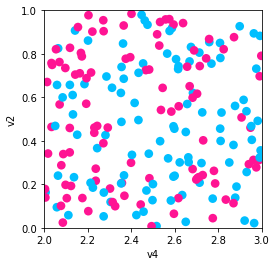
\includegraphics[width=\textwidth]{figures/code/scatter_0.png}
    \end{subfigure}
    \begin{subfigure}{0.5\textwidth}
        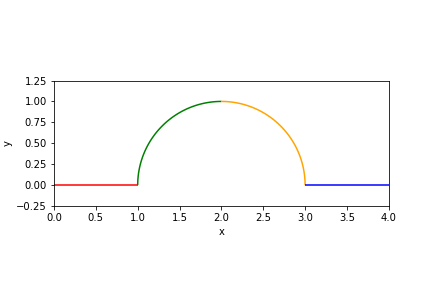
\includegraphics[width=\textwidth]{figures/code/line_1.png}
    \end{subfigure}
    \caption{Scatter plot and line plot implemented using prototype artists and data models, building on Matplotlib rendering.}
    \label{fig:code_scatter_line}
\end{figure}

To prototype our model, we implemented the artist classes for the scatter and line plots shown in figure~\ref{fig:code_scatter_line} because they differ in every attribute of our artist: different visual channels \vchannel\ that composite to different marks \vmark\ with different continuities \vindex\.  We make use of the Matplotlib figure and axes artists \cite{hunterArchitectureOpenSource,hunterMatplotlib2DGraphics2007} so that we can initially focus on the data to graphic transformations. 

To generate the images in figure~\ref{fig:code_scatter_line}, we instantiate \mintinline{python}{fig, ax} artists that will contain the new \mintinline{python}{Point, Line} primitive objects we implemented based on our topology model. 

\begin{multicols*}{2}
\begin{minted}{python}
    fig, ax = plt.subplots()
    artist = Point(data, transforms)
    ax.add_artist(artist)
\end{minted}
\columnbreak
\begin{minted}{python}
    fig, ax = plt.subplots()
    artist = Line(data, transforms)
    ax.add_artist(artist)
\end{minted}
\end{multicols*}

We then add the \vartisteq=\mintinline{python}{Point} and  \vartisteq=\mintinline{python}{Line} artists that construct the scatter and line graphics. The arguments to the artist are the data \dtotal=\mintinline{python}{data} that is to be plotted and the aesthetic configuration \vchannel=\mintinline{python}{transforms}. We implement the artists as equivalence classes \vartisteq\ because it would be impractical to implement a new artist for every aesthetic setting, such as one artist for red lines and another for green.
 
\subsection{Artist Class $\vartist^{\prime}$}
The artist is the piece of the matplotlib architecture that constructs an internal representation of the graphic that the render then uses to draw the graphic. In the prototype artist, \mintinline{python}{transform} is a dictionary of the form \mintinline{python}|{parameter:(variable, encoder)}| where parameter is a component in \vfiber, variable is a component in \dfiber,  and the \vchannel\ encoders are passed in as functions or callable objects. The data bundle \dtotal\ is passed in as a \mintinline{python}{data} object. By binding data and transforms to \vartisteq\ inside \mintinline{python}{__init__}, the \mintinline{python}{draw} method is a fully specified artist \vartist.

\begin{minted}{python}
class ArtistClass(matplotlib.artist.Artist):
    def __init__(self, data, transforms, *args, **kwargs):
        # properties that are specific to the graphic but not the channels
        self.data = data 
        self.transforms = transforms
        super().__init__(*args, **kwargs)

    def assemble(self, visual):
        # set the properties of each glyph

    def draw(self, renderer, *args, **kwargs):
        # returns K, indexed on fiber then key 
        view = self.data.view() 
        # visual channel encoding applied fiberwise 
        visual = {p: encoder(view.get(f, None)) for 
                     p, (f, encoder) in self.transforms.items()}
        self.assemble(visual)
        # pass configurations off to the render
        super().draw(renderer, *args, **kwargs)
\end{minted}

The data is fetched in section \dsection\ via a \mintinline{python}{view} method n the data because the input to the artist is a section on \dtotal. The return view object has a \mintinline{python}{get} method to support querying for components that are not in \dfiber\, which we exploit to support parameters in the visual fiber that are not bound to fiber components in \dfiber. The \vchannel\ functions are then applied to the data to generate the \vsection=\mintinline{python}{visual} input to \vmark. An explicit \vindex\ is not implemented since that would mean copying a single \vsection on \dbasepoint to all the associated \gbasepoint, as illustrated in figure~\ref{fig:graphic_retraction_map}, and that is unnecessary overhead for these scatter and line plots. In \vmarkd=\mintinline{python}{assemble} the artist generates instructions for the render by setting  the attributes that are related to the graphic. These are the settings that would have to be serialized in order to recreate a static version of the graphic. The \vchannel\ functions could be evaluated in this function to avoid passing over \dbase twice. The last step in the artist function is handing itself off to the renderer. 

The \mintinline{python}{Point} artist builds on \mintinline{python}{collection} artists because collections are optimized to efficiently draw a sequence of simple glyphs. In this prototype, the scatter marker shape is fixed as a circle, and the only visual fiber components are x and y position, size, and the facecolor of the marker. 
\begin{minted}{python}
class Point(mcollections.Collection):
    ## init as described above
    def draw(self, renderer, *args, **kwargs):
        # query data for a vertex table K
        view = self.data.view('vertex') 
        visual = {p: encoder(view.get(f, None)) for
                     p, (f, encoder) in self.transforms.items()}
        # no explicit  S->K since they have the same indexing
        # construct geometries of the circle glyphs in visual coordinates
        self._paths = [mpath.Path.circle(center=(x,y), radius=s) for (x, y, s) 
                in zip(visual['x'],visual['y'], visual['s'])] 
        # set attributes of glyphs, these are vectorized 
        # circles and facecolors are lists of the same size
        self.set_facecolors(visual['facecolors'])
        # call the renderer that will draw based on properties
        super().draw(renderer, *args, **kwargs)
\end{minted} 
The \mintinline{python}{view} method repackages the data as a fiber component indexed table of vertices, as described in section~\ref{sec:triangulization}; even though the \mintinline{python}{view} is fiber indexed, each vertex at an index \dbasepoint has corresponding values in section $\dsection(\dbasepoint_{i})$ such that all the data on one vertex maps to one marker. To ensure the integrity of the section, \mintinline{python}{view} must be atomic, meaning that the values cannot change after the method is called in draw until a new call in draw.

This table is converted to a table of visual variables; it is then used to individually construct the vector path of each circular marker with center \texttt{(x,y)} and size \texttt{x} and set the colors of each circle. Since \mintinline{python}{view} returns a \desection\, all these operations could be applied on one element in the data or multiple. \note{this might be better suited for discussion/future work} We could also rewrite the base \vmark\ such that \mintinline{python}{draw} acts on only one point on \dbase\ or even \gbase\, but for small datasets it is more efficient to vectorize these operations. 

The only difference between the \mintinline{python}{Point} and \mintinline{python}{Line} objects is in the \mintinline{python}{view} and in the \vmark\ section because line has different continuity from scatter.

\begin{minted}{python}
class Line(mcollections.LineCollection):
    def draw(self, renderer, *args, **kwargs):
        view = self.data.view('edge')
        visual = {p: encoder(view.get(f, None)) for 
                      p, (f, encoder) in self.transforms.items()}
        # glyph assembly, where the glyph is a line
        segments = [np.vstack((vx, vy)).T for vx, vy 
                    in zip(visual['x'], visual['y'])]
        self.set_segments(segments)
        self.set_color(visual['color'])

        super().draw(renderer, *args, **kwargs)
\end{minted}
In the \mintinline{python}{Line} artist, \mintinline{python}{view} returns a table of edges. Each edge consists of (x,y) points sampled along the line defined by the edge and information such as the color of the edge. This information is converted into visual variables that are then composed into colored line segments. 

\subsubsection{Encoders \vchannel}
what, why, how?
\subsubsection{Data \dtotal}
what, why, how?

\subsubsection{Case Study: Iris}

\end{document}